\section{Some finite subgroups}

    \subsection{Finite subgroups of $\SU(2)$ and $\SL(2,\C)$}

        \subsubsection{Finite subgroups}

            The first thing to recall is that every finite subgroup of $\SL(2,\C)$ is isomorphic to a subgroup of $\SU(2,\C)$ and vice-versa, so we equivalently talk about the subgroups of $\SU(2)$. The finite subgroups of $\SU(2)$, called the \emph{binary polyhedral groups}, are the doubles covers of the finite subgroups of $\SO(3)$ that are called \emph{polyhedral groups}. They simply constitutes the symmetries of the Platonic solids. The groups fall into two infinite series, associated to the regular polygons, as well as three exceptional, associated with the 5 regular polyhedra: the tetrahedron (self-dual), the cube (and its dual octahedron), the icosahedron (and its dual dodecahedron).

            More precisely, the finite subgroups of $\SL(2,\C)$ are
            \begin{itemize}
                \item $\Z_n$ : cyclic group of order $n$ ($n\geq2$) generated by
                \begin{equation}
                    \begin{bmatrix}
                        \zeta_m & 0\\
                        0 & \zeta^{-1}_m
                    \end{bmatrix}
                \end{equation}
                \item $2\D_n$ : \emph{binary dihedral groups} (also known as the \emph{dicyclic group}) of order $4n$ ($n\geq1$) generated by
                \begin{equation}
                    A \equiv
                    \begin{bmatrix}
                        \zeta_{2n} & 0\\
                        0 & \zeta^{-1}_{2n}
                    \end{bmatrix}\quad \text{ and }
                    B \equiv 
                    \begin{bmatrix}
                        0 & i\\
                        i & 0
                    \end{bmatrix}
                \end{equation}
                One can show that $A^n=B^2$ and that $AB=BA^{-1}$ so that $2\D_n=\{B^bA^a|0\leq b \leq 3, 0\leq a \leq n-1\}$. This rewriting of the most general element of the group will be useful.
                \item $2\mathcal{T}$ : \emph{binary tetrahedral group} of order $24$ generated by $D_2$ and
                \begin{equation}
                    C \equiv \frac{1}{\sqrt{2}}
                    \begin{bmatrix}
                        \zeta_8 & \zeta^3_8\\
                        \zeta_8 & \zeta^7_8
                    \end{bmatrix}
                \end{equation}
                \item $2\mathcal{O}$ : \emph{binary octahedral group} of order $48$ generated by $\mathcal{T}$ and
                \begin{equation}
                    D \equiv 
                    \begin{bmatrix}
                        \zeta^3_8 & 0\\
                        0 & \zeta^5_8
                    \end{bmatrix}
                \end{equation}
                \item $2\mathcal{I}$ : \emph{binary icosahedral group} of order $120$ generated by
                \begin{equation}
                    E \equiv -\frac{1}{\sqrt{5}}
                    \begin{bmatrix}
                        \zeta^4_5-\zeta_5 & \zeta^2_5-\zeta^3_5\\
                        \zeta^2_5-\zeta^3_5 & \zeta_5-\zeta^4_5
                    \end{bmatrix}\quad \text{ and }
                    F \equiv -\frac{1}{\sqrt{5}}
                    \begin{bmatrix}
                        \zeta^2_5-\zeta^4_4 & \zeta^4_5-1\\
                        1-\zeta_5 & \zeta^3_5-\zeta_5
                    \end{bmatrix}
                \end{equation}
            \end{itemize}
            with $\zeta_m\equiv e^{i\frac{2\pi}{m}}$ such that $(\zeta_m)^m=1$. Note that the orders are all divisible by $2$. This is because the center of $\SU(2)$ is $\Z_2$.

        \subsubsection{Irreducible representations}\label{sec:irrep}

            \begin{itemize}
                \item $\Z_n$ has $n$ irreducible representations. They are all $1$-dimensional (since $\Z_n$ is abelian) and are given by
                \begin{equation}
                    \rho_k(g)=\zeta^k_n
                \end{equation}
                with $k=0,\dots,n-1$.
                \item $2\D_n$ has $n+3$ irreducible representations: $4$ of dimension $1$ and $n-1$ of dimension $2$. The $1$-dimensional ones are given by
                \begin{equation*}
                \begin{array}{|c|c|c|c|}
                    \hline
                    n & \rho(A) & \rho(B) & \rho(B^bA^a) \\
                    \hline
                    \multirow[c]{4}{*}{\text{even}} & \multirow[c]{2}{*}{1} & 1 & 1 \\ \cline{3-4}
                    & & -1 & (-1)^b \\ \cline{2-4}
                    & \multirow[c]{2}{*}{-1} & 1 & (-1)^a \\ \cline{3-4}
                    & & -1 & (-1)^{a+b} \\
                    \hline
                    \multirow[c]{4}{*}{\text{odd}} & \multirow[c]{2}{*}{1} & 1 & 1 \\ \cline{3-4}
                    & & -1 & (-1)^b \\ \cline{2-4}
                    & \multirow[c]{2}{*}{-1} & i & (-1)^ai^b \\ \cline{3-4}
                    & & -i & (-1)^a(-i)^b \\
                    \hline
                \end{array}
                \end{equation*}
                and the $2$-dimensional ones are given binary by
                \begin{align*}
                    \rho_r(A) &= 
                    \begin{bmatrix}
                        e^{i\frac{\pi}{n}r} & 0\\
                        0 & e^{-i\frac{\pi}{n}r} 
                    \end{bmatrix}\\
                    \rho_r(B) &= 
                    \begin{bmatrix}
                        0 & (-1)^r \\
                        1 & 0
                    \end{bmatrix}
                \end{align*}
                with $r=1,\dots,n-1$.
            \end{itemize}

        \subsubsection{Character tables}

            \begin{table}[H]
                \centering
                {\small
                \begin{equation*}
                        \begin{array}{|c|c|c|c|c|c|}
                            \hline
                            \text{conj. class repr.} & e & M & M^2 & \dots & M^{n-1} \\ \hline
                            \text{conj. class order} & 1 & 1 & 1 & \dots & 1 \\
                            \hline
                            V_0 & 1 & 1 & 1 & \dots & 1 \\
                            V_1 & 1 & \zeta_n & \zeta^2_n & \dots & \zeta^{n-1}_n \\
                            V_2 & 1 & \zeta^2_n & \zeta^4_n & \dots & \zeta^{2(n-1)}_n \\
                            V_3 & 1 & \zeta^3_n & \zeta^6_n & \dots & \zeta^{3(n-1)}_n \\
                            \vdots & \vdots & \vdots & \vdots & \ddots &  \\
                            V_{n-1} & 1 & \zeta^{(n-1)}_n & \zeta^{2(n-1)}_n & \dots & \zeta^{(n-1)^2}_n \\ \hline
                            W & 2 & 2\cos\left(\frac{2\pi}{n}\right) & 2\cos\left(\frac{4\pi}{n}\right) & \dots & 2\cos\left(\frac{2\pi(n-1)}{n}\right) \\ \hline 
                            \end{array}
                    \end{equation*}}
                \caption{Character table of $\Z_n$.}
            \end{table}

            \begin{table}[H]
                \centering
                {\small
                \begin{equation*}
                        \begin{array}{|c|c|c|c|c|c|c|c|c|}
                            \hline
                            \text{conj. class repr.} & e & B^2 & B & BA & A & A^2 & \dots & A^{n-1} \\ \hline
                            \text{conj. class order} & 1 & 1 & n & n & 2 & 2 & \dots & 2 \\
                            \hline
                            V_0 & 1 & 1 & 1 & 1 & 1 & 1 & \dots & 1 \\ 
                            V_1 & 1 & 1 & -1 & -1 & 1 & 1 & \dots & 1 \\ 
                            V_2 & 1 & 1 \text{ ou } -1 & 1 \text{ ou } i & -1 \text{ ou } -i & -1 & 1 & \dots & (-1)^{n-1} \\ 
                            V_3 & 1 & 1 \text{ ou } -1 & -1 \text{ ou } -i & 1 \text{ ou } i & -1 & 1 & \dots & (-1)^{n-1} \\
                            V_4 & 2 & -2 & 0 & 0 & 2\cos\frac{\pi}{n} & 2\cos\frac{2\pi}{n} & \dots & 2\cos\frac{(n-1)\pi}{n}\\
                            V_5 & 2 & 2 & 0 & 0 & 2\cos\frac{2\pi}{n} & 2\cos\frac{4\pi}{n} & \dots & 2\cos\frac{2(n-1)\pi}{n}\\
                            \vdots & \vdots & \vdots & \vdots & \vdots & \vdots & \vdots & \ddots & \vdots \\
                            V_{n+2} & 2 & 2(-1)^{n-1} & 0 & 0 & 2\cos\frac{(n-1)\pi}{n} & 2\cos\frac{2(n-1)\pi}{n} & \dots & 2\cos\frac{(n-1)^2\pi}{n} \\ \hline
                            W & 2 & -2 & 0 & 0 & 2\cos\left(\frac{\pi}{n}\right) & 2\cos\left(2\frac{\pi}{n}\right) & \dots & 2\cos\left(\frac{\pi}{n}(n-1)\right) \\ \hline
                            \end{array}
                    \end{equation*}}
                \caption{Character table of $2\D_n$.}
            \end{table}

            \begin{table}[H]
                \centering
                {\small
                \begin{equation*}
                        \begin{array}{|c|c|c|c|c|c|c|c|}
                            \hline
                            \text{conj. class repr.} & e & B^2 & B & C & C^2 & C^4 & C^5 \\ \hline
                            \text{conj. class order} & 1 & 1 & 6 & 4 & 4 & 4 & 4\\
                            \hline
                            V_0 & 1 & 1 & 1 & 1 & 1 & 1 & 1 \\
                            V_1 & 2 & -2 & 0 & 1 & -1 & -1 & 1 \\
                            V_2 & 3 & 3 & -1 & 0 & 0 & 0 & 0 \\
                            V_3 & 2 & -2 & 0 & e^{i\frac{2\pi}{3}} & -e^{i\frac{2\pi}{3}} & -e^{i\frac{4\pi}{3}} & e^{i\frac{4\pi}{3}} \\
                            V_3^{\lor} & 2 & -2 & 0 & e^{i\frac{4\pi}{3}} & -e^{i\frac{4\pi}{3}} & -e^{i\frac{2\pi}{3}} & e^{i\frac{2\pi}{3}} \\
                            V_4 & 1 & 1 & 1 & e^{i\frac{2\pi}{3}} & e^{i\frac{2\pi}{3}} & e^{i\frac{4\pi}{3}} & e^{i\frac{4\pi}{3}} \\
                            V_4^{\lor} & 1 & 1 & 1 & e^{i\frac{4\pi}{3}} & e^{i\frac{4\pi}{3}} & e^{i\frac{2\pi}{3}} & e^{i\frac{2\pi}{3}} \\ \hline
                            W & 2 & -2 & 0 & 1 & -1 & -1 & 1 \\ \hline
                        \end{array}
                    \end{equation*}}
                \caption{Character table of $2\mathcal{T}$.}
            \end{table}

            \begin{table}[H]
                \centering
                {\small
                \begin{equation*}
                        \begin{array}{|c|c|c|c|c|c|c|c|c|}
                            \hline
                            \text{conj. class repr.} & e & B^2 & B & C & C^2 & D & BD & D^3 \\ \hline
                            \text{conj. class order} & 1 & 1 & 6 & 8 & 8 & 6 & 12 & 6\\
                            \hline
                            V_0 & 1 & 1 & 1 & 1 & 1 & 1 & 1 & 1 \\
                            V_1 & 2 & -2 & 0 & 1 & -1 & -\sqrt{2} & 0 & \sqrt{2} \\
                            V_2 & 3 & 3 & -1 & 0 & 0 & 1 & -1 & 1 \\
                            V_3 & 4 & -4 & 0 & -1 & 1 & 0 & 0 & 0 \\
                            V_4 & 3 & 3 & -1 & 0 & 0 & -1 & 1 & -1 \\
                            V_5 & 2 & -2 & 0 & 1 & -1 & \sqrt{2} & 0 & -\sqrt{2} \\
                            V_6 & 1 & 1 & 1 & 1 & 1 & -1 & -1 & -1 \\
                            V_7 & 2 & 2 & 2 & -1 & -1 & 0 & 0 & 0 \\ \hline
                            W & 2 & -2 & 0 & 1 & -1 & -\sqrt{2} & 0 & \sqrt{2} \\ \hline
                        \end{array}
                    \end{equation*}}
                \caption{Character table of $2\mathcal{O}$.}
            \end{table}

            \begin{table}[H]
                \centering
                {\small
                \begin{equation*}
                        \begin{array}{|c|c|c|c|c|c|c|c|c|c|}
                            \hline
                            \text{conj. class repr.} & e & E^2 & E & F & F^2 & EF & (EF)^2 & (EF)^3 & (EF)^4 \\ \hline
                            \text{conj. class order} & 1 & 1 & 30 & 20 & 20 & 12 & 12 & 12 & 12\\
                            \hline
                            V_0 & 1 & 1 & 1 & 1 & 1 & 1 & 1 & 1 & 1 \\
                            V_1 & 2 & -2 & 0 & 1 & -1 & \vp^+ & -\vp^- & \vp^- & -\vp^+ \\
                            V_2 & 3 & 3 & -1 & 0 & 0 & \vp^+ & \vp^- & \vp^- & \vp^+ \\
                            V_3 & 4 & -4 & 0 & -1 & 1 & 1 & -1 & 1 & -1 \\
                            V_4 & 5 & 5 & 1 & -1 & -1 & 0 & 0 & 0 & 0 \\
                            V_5 & 6 & -6 & 0 & 0 & 0 & -1 & 1 & -1 & 1 \\
                            V_6 & 4 & 4 & 0 & 1 & 1 & -1 & -1 & -1 & -1 \\
                            V_7 & 2 & -2 & 0 & 1 & -1 & \vp^- & -\vp^+ & \vp^+ & -\vp^- \\
                            V_8 & 3 & 3 & -1 & 0 & 0 & \vp^- & \vp^+ & \vp^+ & \vp^- \\ \hline
                            W & 2 & -2 & 0 & 1 & -1 & \vp^+ & -\vp^- & \vp^- & -\vp^+ \\ \hline
                        \end{array}
                    \end{equation*}}
                \caption{Character table of $2\mathcal{I}$, with $\vp^\pm\equiv(1\pm\sqrt{5})/2$.}
            \end{table}


    \subsection{Finite subgroups of $\SU(3)$}

        The finite subgroups of $\SU(3)$ are
        \begin{itemize}
            \item the finite subgroups of $\SU(2)$
        \end{itemize}
        so there are $2$ infinite series and $5$ exceptional subgroups. Note that they are all divisible by $3$ because the center of $\SU(3)$ is $\Z_3$.

\section{The McKay correspondence}\label{app:McKay}

    \subsection{Classical correspondence}

        \begin{table}[H]
            \centering
            \begin{tabular}{|c|l|l|l|}
                \hline
                $\Gamma\subset\SU(2)$ & Platonic solids & McKay graph & Variety \\ \hline
                $\Z_n$ &  & \begin{tikzpicture}[baseline={($ (current bounding box.center) - (0,3pt) $)},scale=0.5]
                    \draw (0,0) edge (2*1.25,0);
                    \draw (2*1.25,0) edge[dashed] (3*1.25,0);
                    \draw (3*1.25,0) edge (4*1.25,0);
                    \draw (0,0) edge (2*1.25,-1);
                    \draw (4*1.25,0) edge (2*1.25,-1);
                    \foreach \x in {0,1,2,3,4} {
                        \draw[fill=black] (1.25*\x,0) circle[radius=0.15];
                        \draw (1.25*\x,0) node[above]{$1$};
                    }
                    \draw[fill=black] (1.25*2,-1) circle[radius=0.15];
                    \draw (1.25*2,-1) node[above]{$1$};
                \end{tikzpicture}\quad($n$ nodes) & $z^{n}+xy=0$ \\ \hline
                $2\mathcal{D}_n$ & $n$-polygon & \begin{tikzpicture}[baseline={($ (current bounding box.center) - (0,3pt) $)},scale=0.5]
                    \draw (0,0) edge (2*1.25,0);
                    \draw (2*1.25,0) edge[dashed] (3*1.25,0);
                    \draw (3*1.25,0) edge (4*1.25,0);
                    \draw (4*1.25,0) edge (5*1.25,0);
                    \draw (1.25,0) edge (1.25,-1.25);
                    \draw (4*1.25,0) edge (4*1.25,-1.25);
                    \foreach \x in {0,1,2,3,4,5} {
                        \draw[fill=black] (1.25*\x,0) circle[radius=0.15];
                    }
                    
                    \draw[fill=black] (1.25,-1.25) circle[radius=0.15];
                    \draw (1.25,-1.25) node[right]{$1$};
                    \draw[fill=black] (4*1.25,-1.25) circle[radius=0.15];
                    \draw (4*1.25,-1.25) node[right]{$1$};
                    \draw (0,0) node[above]{$1$};
                    \draw (1.25*5,0) node[above]{$1$};
                    \draw (1.25*1,0) node[above]{$2$};
                    \draw (1.25*2,0) node[above]{$2$};
                    \draw (1.25*3,0) node[above]{$2$};
                    \draw (1.25*4,0) node[above]{$2$};
                \end{tikzpicture}\quad($n+3$ nodes) & $x^2+y^2z+z^{n-1}=0$ \\ \hline
                $2\mathcal{T}$ & tetrahedron & \begin{tikzpicture}[baseline={($ (current bounding box.center) - (0,3pt) $)},scale=0.5]
                    \draw (0,0) edge (4*1.25,0);
                    \draw (2*1.25,0) edge (2*1.25,-2*1.25);
                    \foreach \x in {0,1,2,3,4} {
                        \draw[fill=black] (1.25*\x,0) circle[radius=0.15];
                    }
                    \draw[fill=black] (2*1.25,-1.25) circle[radius=0.15];
                    \draw (2*1.25,-1.25) node[right]{$2$};
                    \draw[fill=black] (2*1.25,-2*1.25) circle[radius=0.15];
                    \draw (2*1.25,-2*1.25) node[right]{$1$};
                    \draw (0,0) node[above]{$1$};
                    \draw (1.25*4,0) node[above]{$1$};
                    \draw (1.25*1,0) node[above]{$2$};
                    \draw (1.25*2,0) node[above]{$3$};
                    \draw (1.25*3,0) node[above]{$2$};
                \end{tikzpicture}\quad($7$ nodes) & $x^2+y^3+z^4=0$ \\ \hline
                $2\mathcal{O}$  & \begin{tabular}{@{}l@{}}cube \\ octahedron\end{tabular} & \begin{tikzpicture}[baseline={($ (current bounding box.center) - (0,3pt) $)},scale=0.5]
                    \draw (0,0) edge (6*1.25,0);
                    \draw (3*1.25,0) edge (3*1.25,-1.25);
                    \foreach \x in {0,1,2,3,4,5,6} {
                        \draw[fill=black] (1.25*\x,0) circle[radius=0.15];
                    }
                    \draw[fill=black] (3*1.25,-1.25) circle[radius=0.15];
                    \draw (3*1.25,-1.25) node[right]{$2$};
                    \draw (0,0) node[above]{$1$};
                    \draw (1.25*1,0) node[above]{$2$};
                    \draw (1.25*2,0) node[above]{$3$};
                    \draw (1.25*3,0) node[above]{$4$};
                    \draw (1.25*4,0) node[above]{$3$};
                    \draw (1.25*5,0) node[above]{$2$};
                    \draw (1.25*6,0) node[above]{$1$};
                \end{tikzpicture}\quad($8$ nodes) & $x^2+y^3+yz^3=0$ \\ \hline
                $2\mathcal{I}$  & \begin{tabular}{@{}l@{}}icosahedron \\ dodecahedron\end{tabular} & \begin{tikzpicture}[baseline={($ (current bounding box.center) - (0,3pt) $)},scale=0.5]
                    \draw (0,0) edge (7*1.25,0);
                    \draw (2*1.25,0) edge (2*1.25,-1.25);
                    \foreach \x in {0,1,2,3,4,5,6,7} {
                        \draw[fill=black] (1.25*\x,0) circle[radius=0.15];
                    }
                    \draw[fill=black] (2*1.25,-1.25) circle[radius=0.15];
                    \draw (2*1.25,-1.25) node[right]{$3$};
                    \draw (0,0) node[above]{$2$};
                    \draw (1.25*1,0) node[above]{$4$};
                    \draw (1.25*2,0) node[above]{$6$};
                    \draw (1.25*3,0) node[above]{$5$};
                    \draw (1.25*4,0) node[above]{$4$};
                    \draw (1.25*5,0) node[above]{$3$};
                    \draw (1.25*6,0) node[above]{$2$};
                    \draw (1.25*7,0) node[above]{$1$};
                \end{tikzpicture}\quad($9$ nodes) & $x^2+y^3+z^5=0$ \\ \hline
            \end{tabular}
            \caption{Binary polyhedral groups and their McKay graphs.Labels over the vertices are the dimension of the representation. We erase the arrow ends if they go in both directions and erase the label if it is
            equal to $1$.}
        \end{table}

        \begin{figure}[H]
            \centering
            \begin{tabular}{|c|c|l|}
                \hline
                \begin{tabular}{@{}c@{}}Simple \\ Lie algebra\end{tabular} & Simply laced & \begin{tabular}{@{}l@{}}Dynkin diagram \\ Extended Dybkin diagram\end{tabular} \\ \hline
                $\mathfrak{sl}(n+1,\C),n\geq1$ & yes & 
                \begin{tabular}{@{}l@{}} $A_n:\quad$ \begin{tikzpicture}[baseline={($ (current bounding box.center) - (0,3pt) $)},scale=0.5]
                    \draw (0,0) edge (2*1.25,0);
                    \draw (2*1.25,0) edge[dashed] (3*1.25,0);
                    \draw (3*1.25,0) edge (4*1.25,0);
                    \foreach \x in {0,1,2,3,4} {
                    \draw[fill=white] (1.25*\x,0) circle[radius=0.15];
                    }
                    \end{tikzpicture}\quad($n$ nodes) \\[0.4cm] $\tilde{A}_n:\quad$ \begin{tikzpicture}[baseline={($ (current bounding box.center) - (0,3pt) $)},scale=0.5]
                        \draw (0,0) edge (2*1.25,0);
                        \draw (2*1.25,0) edge[dashed] (3*1.25,0);
                        \draw (3*1.25,0) edge (4*1.25,0);
                        \draw (0,0) edge (2*1.25,1);
                        \draw (4*1.25,0) edge (2*1.25,1);
                        \foreach \x in {0,1,2,3,4} {
                            \draw[fill=white] (1.25*\x,0) circle[radius=0.15];
                        }
                        \draw[fill=black] (1.25*2,1) circle[radius=0.15];
                    \end{tikzpicture}\quad($n+1$ nodes)\end{tabular} \\ \hline
                $\mathfrak{so}(2n+1,\R),n\geq2$ & no & 
                \begin{tabular}{@{}l@{}}$B_n:\quad$ \begin{tikzpicture}[baseline={($ (current bounding box.center) - (0,3pt) $)},scale=0.5]
                    \draw (0,0) edge (2*1.25,0);
                    \draw (2*1.25,0) edge[dashed] (3*1.25,0);
                    \draw (3*1.25+0.65-0.15,0.21) -- (3*1.25+0.65+0.15,0) -- (3*1.25+0.65-0.15,-0.21);
                    \draw (3*1.25,0.07) -- (4*1.25,0.07);
                    \draw (3*1.25,-0.07) -- (4*1.25,-0.07); 
                    \foreach \x in {0,1,2,3,4} {
                    \draw[fill=white] (1.25*\x,0) circle[radius=0.15];
                    }
                    \end{tikzpicture}\quad ($n$ nodes) \\[0.4cm] $\tilde{B}_n:\quad$ \begin{tikzpicture}[baseline={($ (current bounding box.center) - (0,3pt) $)},scale=0.5]
                        \draw (1.25,0) edge (2*1.25,0);
                        \draw (0,0.7) edge (1.25,0);
                        \draw (0,-0.7) edge (1.25,0);
                        \draw (2*1.25,0) edge[dashed] (3*1.25,0);
                        \draw (3*1.25+0.65-0.15,0.21) -- (3*1.25+0.65+0.15,0) -- (3*1.25+0.65-0.15,-0.21);
                        \draw (3*1.25,0.07) -- (4*1.25,0.07);
                        \draw (3*1.25,-0.07) -- (4*1.25,-0.07); 
                        \foreach \x in {1,2,3,4} {
                            \draw[fill=white] (1.25*\x,0) circle[radius=0.15];
                        }
                        \draw[fill=white] (0,0.7) circle[radius=0.15];
                        \draw[fill=black] (0,-0.7) circle[radius=0.15];
                    \end{tikzpicture}\quad($n+1$ nodes)\end{tabular} \\ \hline
                $\mathfrak{sp}(2n,\C),n\geq3$ & no & 
                \begin{tabular}{@{}l@{}}$C_n:\quad$ \begin{tikzpicture}[baseline={($ (current bounding box.center) - (0,4pt) $)},scale=0.5]
                    \draw (0,0) edge (2*1.25,0);
                    \draw (2*1.25,0) edge[dashed] (3*1.25,0);
                    \draw (3*1.25+0.65+0.15,0.21) -- (3*1.25+0.65-0.15,0) -- (3*1.25+0.65+0.15,-0.21);
                    \draw (3*1.25,0.07) -- (4*1.25,0.07);
                    \draw (3*1.25,-0.07) -- (4*1.25,-0.07); 
                    \foreach \x in {0,1,2,3,4} {
                    \draw[fill=white] (1.25*\x,0) circle[radius=0.15];
                    }
                    \end{tikzpicture}\quad ($n$ nodes) \\[0.4cm] $\tilde{C}_n:\quad$ \begin{tikzpicture}[baseline={($ (current bounding box.center) - (0,4pt) $)},scale=0.5]
                        \draw (0.65-0.15,0.21) -- (0.65+0.15,0) -- (0.65-0.15,-0.21);
                        \draw (0,0.07) -- (1.25,0.07);
                        \draw (0,-0.07) -- (1.25,-0.07);
                        \draw (1.25,0) edge (2*1.25,0);
                        \draw (2*1.25,0) edge[dashed] (3*1.25,0);
                        \draw (3*1.25+0.65+0.15,0.21) -- (3*1.25+0.65-0.15,0) -- (3*1.25+0.65+0.15,-0.21);
                        \draw (3*1.25,0.07) -- (4*1.25,0.07);
                        \draw (3*1.25,-0.07) -- (4*1.25,-0.07); 
                        \foreach \x in {1,2,3,4} {
                            \draw[fill=white] (1.25*\x,0) circle[radius=0.15];
                        }
                        \draw[fill=black] (0,0) circle[radius=0.15];
                    \end{tikzpicture}\quad($n+1$ nodes)\end{tabular} \\ \hline
                $\mathfrak{so}(2n,\R),n\geq4$ & yes &
                \begin{tabular}{@{}l@{}}$D_n:\quad$ \begin{tikzpicture}[baseline={($ (current bounding box.center) - (0,3pt) $)},scale=0.5]
                    \draw (0,0) edge (2*1.25,0);
                    \draw (2*1.25,0) edge[dashed] (3*1.25,0);
                    \draw (3*1.25,0) -- (4*1.25,0.7);
                    \draw (3*1.25,0) -- (4*1.25,-0.7); 
                    \foreach \x in {0,1,2,3} {
                    \draw[fill=white] (1.25*\x,0) circle[radius=0.15];
                    }
                    \draw[fill=white] (1.25*4,0.7) circle[radius=0.15];
                    \draw[fill=white] (1.25*4,-0.7) circle[radius=0.15];
                    \end{tikzpicture}\quad($n$ nodes) \\[0.4cm] $\tilde{D}_n:\quad$  \begin{tikzpicture}[baseline={($ (current bounding box.center) - (0,3pt) $)},scale=0.5]
                        \draw (0,0.7) edge (1.25,0);
                        \draw (0,-0.7) edge (1.25,0);
                        \draw (1.25,0) edge (2*1.25,0);
                        \draw (2*1.25,0) edge[dashed] (3*1.25,0);
                        \draw (3*1.25,0) -- (4*1.25,0.7);
                        \draw (3*1.25,0) -- (4*1.25,-0.7); 
                        \foreach \x in {1,2,3} {
                            \draw[fill=white] (1.25*\x,0) circle[radius=0.15];
                        }
                        \draw[fill=white] (0,0.7) circle[radius=0.15];
                        \draw[fill=black] (0,-0.7) circle[radius=0.15];
                        \draw[fill=white] (1.25*4,0.7) circle[radius=0.15];
                        \draw[fill=white] (1.25*4,-0.7) circle[radius=0.15];
                    \end{tikzpicture}\quad($n+1$ nodes)\end{tabular} \\ \hline
                $\mathfrak{e}_6$ & yes &
                \begin{tabular}{@{}l@{}}$E_6:\quad$ \begin{tikzpicture}[baseline={($ (current bounding box.south) + (0,1pt) $)},scale=0.5]
                    \draw (0,0) edge (4*1.25,0);
                    \draw (2*1.25,0) edge (2*1.25,1.25);
                    \foreach \x in {0,1,2,3,4} {
                    \draw[fill=white] (1.25*\x,0) circle[radius=0.15];
                    }
                    \draw[fill=white] (2*1.25,1.25) circle[radius=0.15];
                    \end{tikzpicture} \quad($6$ nodes) \\[0.4cm]  $\tilde{E}_6:\quad$ \begin{tikzpicture}[baseline={($ (current bounding box.south) + (0,1pt) $)},scale=0.5]
                        \draw (0,0) edge (4*1.25,0);
                        \draw (2*1.25,0) edge (2*1.25,2*1.25);
                        \foreach \x in {0,1,2,3,4} {
                            \draw[fill=white] (1.25*\x,0) circle[radius=0.15];
                        }
                        \draw[fill=white] (2*1.25,1.25) circle[radius=0.15];
                        \draw[fill=black] (2*1.25,2*1.25) circle[radius=0.15];
                    \end{tikzpicture}\quad($7$ nodes)\end{tabular} \\ \hline
                $\mathfrak{e}_7$ & yes & 
                \begin{tabular}{@{}l@{}} $E_7:\quad$ \begin{tikzpicture}[baseline={($ (current bounding box.south) + (0,1pt) $)},scale=0.5]
                    \draw (0,0) edge (5*1.25,0);
                    \draw (2*1.25,0) edge (2*1.25,1.25);
                    \foreach \x in {0,1,2,3,4,5} {
                    \draw[fill=white] (1.25*\x,0) circle[radius=0.15];
                    }
                    \draw[fill=white] (2*1.25,1.25) circle[radius=0.15];
                    \end{tikzpicture} \quad($7$ nodes) \\[0.4cm] $\tilde{E}_7:\quad$ \begin{tikzpicture}[baseline={($ (current bounding box.south) + (0,1pt) $)},scale=0.5]
                        \draw (-1.25,0) edge (5*1.25,0);
                        \draw (2*1.25,0) edge (2*1.25,1.25);
                        \foreach \x in {0,1,2,3,4,5} {
                            \draw[fill=white] (1.25*\x,0) circle[radius=0.15];
                        }
                        \draw[fill=black] (-1.25,0) circle[radius=0.15];
                        \draw[fill=white] (2*1.25,1.25) circle[radius=0.15];
                    \end{tikzpicture}\quad($8$ nodes)\end{tabular} \\ \hline
                $\mathfrak{e}_8$ & yes & 
                \begin{tabular}{@{}l@{}}$E_8:\quad$ \begin{tikzpicture}[baseline={($ (current bounding box.south) + (0,1pt) $)},scale=0.5]
                    \draw (0,0) edge (6*1.25,0);
                    \draw (2*1.25,0) edge (2*1.25,1.25);
                    \foreach \x in {0,1,2,3,4,5,6} {
                    \draw[fill=white] (1.25*\x,0) circle[radius=0.15];
                    }
                    \draw[fill=white] (2*1.25,1.25) circle[radius=0.15];
                    \end{tikzpicture} \quad($8$ nodes) \\[0.4cm] $\tilde{E}_8:\quad$ \begin{tikzpicture}[baseline={($ (current bounding box.south) + (0,1pt) $)},scale=0.5]
                        \draw (0,0) edge (7*1.25,0);
                        \draw (2*1.25,0) edge (2*1.25,1.25);
                        \foreach \x in {0,1,2,3,4,5,6} {
                            \draw[fill=white] (1.25*\x,0) circle[radius=0.15];
                        }
                        \draw[fill=black] (7*1.25,0) circle[radius=0.15];
                        \draw[fill=white] (2*1.25,1.25) circle[radius=0.15];
                    \end{tikzpicture}\quad($9$ nodes)\end{tabular} \\ \hline
                $\mathfrak{f}_4$ & no & 
                \begin{tabular}{@{}l@{}}$F_4:\quad$ \begin{tikzpicture}[baseline={($ (current bounding box.center) - (0,3pt) $)},scale=0.5]
                    \draw (0,0) edge (1.25,0);
                    \draw (2*1.25,0) edge (3*1.25,0);
                    \draw (1*1.25+0.65-0.15,0.21) -- (1*1.25+0.65+0.15,0) -- (1*1.25+0.65-0.15,-0.21);
                    \draw (1*1.25,0.07) -- (2*1.25,0.07);
                    \draw (1*1.25,-0.07) -- (2*1.25,-0.07); 
                    \foreach \x in {0,1,2,3} {
                    \draw[fill=white] (1.25*\x,0) circle[radius=0.15];
                    }
                    \end{tikzpicture} \quad($4$ nodes) \\[0.4cm] $\tilde{F}_4:\quad$  \begin{tikzpicture}[baseline={($ (current bounding box.center) - (0,3pt) $)},scale=0.5]
                        \draw (-1.25,0) edge (1.25,0);
                        \draw (2*1.25,0) edge (3*1.25,0);
                        \draw (1*1.25+0.65-0.15,0.21) -- (1*1.25+0.65+0.15,0) -- (1*1.25+0.65-0.15,-0.21);
                        \draw (1*1.25,0.07) -- (2*1.25,0.07);
                        \draw (1*1.25,-0.07) -- (2*1.25,-0.07); 
                        \foreach \x in {0,1,2,3} {
                            \draw[fill=white] (1.25*\x,0) circle[radius=0.15];
                        }
                        \draw[fill=black] (-1.25,0) circle[radius=0.15];
                    \end{tikzpicture}\quad($5$ nodes)\end{tabular} \\ \hline
                $\mathfrak{g}_2$ & no & 
                \begin{tabular}{@{}l@{}} $G_2:\quad$  \begin{tikzpicture}[baseline={($ (current bounding box.center) - (0,3pt) $)},scale=0.5]
                    \draw (0,0) edge (1.25,0);
                    \draw (0.65-0.15,0.21) -- (0.65+0.15,0) -- (0.65-0.15,-0.21);
                    \draw (0,0.11) -- (1.25,0.11);
                    \draw (0,-0.11) -- (1.25,-0.11); 
                    \foreach \x in {0,1} {
                    \draw[fill=white] (1.25*\x,0) circle[radius=0.15];
                    }
                    \end{tikzpicture} \quad($2$ nodes) \\[0.4cm] $\tilde{G}_2:\quad$ \begin{tikzpicture}[baseline={($ (current bounding box.center) - (0,3pt) $)},scale=0.5]
                        \draw (-1.25,0) edge (1.25,0);
                        \draw (0.65-0.15,0.21) -- (0.65+0.15,0) -- (0.65-0.15,-0.21);
                        \draw (0,0.11) -- (1.25,0.11);
                        \draw (0,-0.11) -- (1.25,-0.11); 
                        \foreach \x in {0,1} {
                            \draw[fill=white] (1.25*\x,0) circle[radius=0.15];
                        }
                        \draw[fill=black] (-1.25,0) circle[radius=0.15];
                    \end{tikzpicture}\quad($3$ nodes)\end{tabular} \\ \hline
            \end{tabular}
            \caption{Simple Lie algebras and their (extended) Dynkin diagrams. The first four algebras are the classical simple Lie algebras and the last five are the excpetional simple Lie algebras.}
        \end{figure}

        Finally, we can see the following correspondence between the extended Dynkin diagrams and the McKay graphs.

        \begin{figure}[H]
            \centering
            \begin{tabular}{|c|c|c|c|c|}
                \hline
                \begin{tabular}{@{}c@{}} Simply Lie \\ group \end{tabular} & \begin{tabular}{@{}c@{}} Simply laced \\ Lie algebra \end{tabular} & \begin{tabular}{@{}c@{}} Extended \\ Dybkin diagram \end{tabular} & \begin{tabular}{@{}c@{}} Finite subgroup \\ of $\SO(3)$ \end{tabular} & \begin{tabular}{@{}c@{}} Finite subgroup \\ of $\SU(2)$ \end{tabular} \\ \hline
                $\SU(n+1)$ & $\mathfrak{sl}(n+1,\C)$ & $\tilde{A}_n$ & $\Z_{n+1}$ & $\Z_{n+1}$ \\ \hline
                $\SO(2n),\Spin(2n)$ & $\mathfrak{so}(2,\R)$ & $\tilde{D}_n$ & $\D_{2(n-2)}$ & $2\D_{2(n-2)}$ \\ \hline
                $E6$ & $\mathfrak{e}_6$ & $\tilde{E_6}$ &  $\T$ & $2\T$ \\ \hline
                $E7$ & $\mathfrak{e}_7$ & $\tilde{E_7}$ & $\O$ & $2\O$ \\ \hline
                $E8$ & $\mathfrak{e}_8$ & $\tilde{E_8}$ & $\I$ & $2\I$ \\ \hline
            \end{tabular}
            \caption{Classical McKay correspondence.}
        \end{figure}

    \subsection{Geometrical McKay correspondence}

\section{Graphs}

    The \emph{dimer diagram} of a quiver gauge theory is a graph whose faces represent the gauge groups, the edges represent the bi-fundamental fields and the vertices represent the superpotentials.

\section{Determinantal varieties as transverse spaces}

    \subsection{Basic properties of determinantal varieties}  

            A \emph{determinantal variety} (DV) is a space of matrices with a given upper bound on their ranks. More precisely, given $m,n$ and $r<\min(m,n)$, the DV $Y_r$ of the field $K$ is the set of $m\times n$ matrices over $K$ with rank lower or equal to $r$:
            \begin{equation}
                Y_r\equiv\{M\in M_{m\times n}(K)|\rank M\leq r\}.
            \end{equation}
            Recall that a $k$-minor is the determinant of a $k\times k$ sub-matrix and that the rank of a matrix is equal to the biggest integer such that there is a non-vanishing minor of that size. Imposing $\rank M\leq r$ is therefore equivalent to the vanishing of its $(r+1)\times (r+1)$ minors, as it also implies tha vanishing of the biggest minors. This naturally qualifies $R_r$ as affine varieties embedded in $K^{mn}$. 
            
            Let us denote by $X=(x_{ij})$ an arbitrary $m\times n$ matrix. The independent entries $x_{ij}$ are affine coordinates. The $(r+1)\times(r+1)$ minors are therefore homogeneous polynomials of degree $r+1$. The \emph{determinantal ideal} $I_{r+1}(X)$ is the ideal of $k[X]$ generated by these polynomials. The cooridnate ring is 
            \begin{equation}
                R=k[X]/I_{r+1}(X)
            \end{equation}
            Homogeneity the polynomials implies that $Y_r$ can equivalently be seen as a projective variety in $\bbA^{mn-1}$.

        \subsubsection{Computing the dimension}
            
            Let us compute the dimension of $Y_r$ seen as an affine variety. We consider the space $\bbA^{mn}\times\textbf{Gr}(r,m)$, where $\textbf{Gr}(r,m)$ is the Grassmannian of $r$-planes in an $m$-dimensioanl vector space. Let us define the subsapce
            \begin{equation}
                Z_r\equiv\{(A,W)|Ax\in W\text{ for all } x\in\bbA^{n}\}.
            \end{equation}
            $Y_r$ and $Z_r$ are birationaly equivalent so $\dim Y_r=\dim Z_r$. We want to compute $Z_r$. First we notice that $Z_r$ is a vector bundle over $\textbf{Gr}(r,m)$ and we denote it by $Z_r\xrightarrow[]{\pi_1}\textbf{Gr}(r,m)$. Now, over the Grassmannian $\textbf{Gr}(r,m)$, there is a tautologial vector bundle that we denote by $E_{\textbf{Gr}}\xrightarrow[]{\pi_2}\textbf{Gr}(r,m)$ whose fibers are $\pi^{-1}_2(W)=W\cong\R^r$. Finally, $K^m$ can also be seen as a vector bundle, with fibers $\R^m$. We denote it by $E_{K^n}\xrightarrow[]{\pi_3}K^n$. From $E_{\textbf{Gr}}$ and $E_{K^n}$, we can construct\footnote{Recall that if $E$ and $F$ are vector bundles over $X$, then we can construct a new vetor bundle over $X$, called the Hom-bundle and denoted $\Hom(E,F)$, by defining the fiber over $x\in X$ to be $\Hom(E_x,F_x)$.} the vector bundle $\Hom(E_{\textbf{Gr}},E_{K^n})\xrightarrow[]{\pi_4}\textbf{Gr}(r,m)$. This vector bundle has the same base space and its fibers are $\Hom(\R^m,\R^r)$ which are exactly the same as the ones of $Z_r$. So the two vector bundles are isomorphic:
            \begin{equation}
                Z_r\cong\Hom(E_{\textbf{Gr}},E_{K^n}).
            \end{equation}
            Finally, since the fibers of $\Hom(K^n,E_{\textbf{Gr}})$ have dimension $nr$, we find
            \begin{equation}
                \dim Z_r = \dim\Hom(K^n,E_{\textbf{Gr}}) = \dim\textbf{Gr}(r,m)+nr = r(m-r)+nr.
            \end{equation}
            Finally, we conclude that $Y_r$ is a affine variety of dimension $r(m-r)+nr$.

            \begin{table}[H]
                \centering
                $
                \begin{array}{|c|c|c||c|}
                    \hline
                    m & n & r & \dim_\C Y_r \\ \hline
                    2 & 2 & 1 & 3 \\ \hline
                    3 & 2 & 1 & 4 \\ \hline
                    3 & 3 & 1 & 5 \\ \hline
                    3 & 3 & 2 & 8 \\ \hline
                    4 & 2 & 1 & 5 \\ \hline
                    4 & 3 & 1 & 6 \\ \hline
                    4 & 3 & 2 & 10 \\ \hline
                    4 & 4 & 1 & 7 \\ \hline
                    4 & 4 & 2 & 12 \\ \hline
                    4 & 4 & 3 & 15 \\ \hline
                \end{array}
                $
            \end{table}

        \subsubsection{Singularity}
        
            Determinantal varieties are singular and possess non-commutative resolutions. $Y_r$ is singlar and the singular locus is contained in the subset of matrices with rank strictly lower than $r$. $Z_r$ is a resolution (over the open set of matrices with rank exactly $r$, this map is an isomorphism), it is called the \emph{Springer desingularization} of $\text{Spec}R$.

        \subsubsection{Action and syzygies}

            $Y_r$ naturally acts on $G=\GL(m,K)\times\GL(n,K)$

        \subsection{Young's lattice}

            \emph{Young's lattice} is a lattice $Y$ formed by all integer partitions ordered by inclusion of their Young tableau. It is generally used to to describe the irreducible representation sof the symmetric group\footnote{Two permutations of $S_n$ are equivalent if and only they have they have the same number of cycles of the same sizes. Therefore, the quivalence classes of the symmetric group $S_n$ are parametrized by the partitions of $n$, i.e. by Young diagrams.} $S_n$ together with their branching properties. Conventionnally, Young's lattice is depicted in a Hasse diagram, i.e. with element of the same rank shown at the same height and with links such that the descendance of two elements is the union and the parent is the intersection.

            \begin{figure}[H]
                \centering
                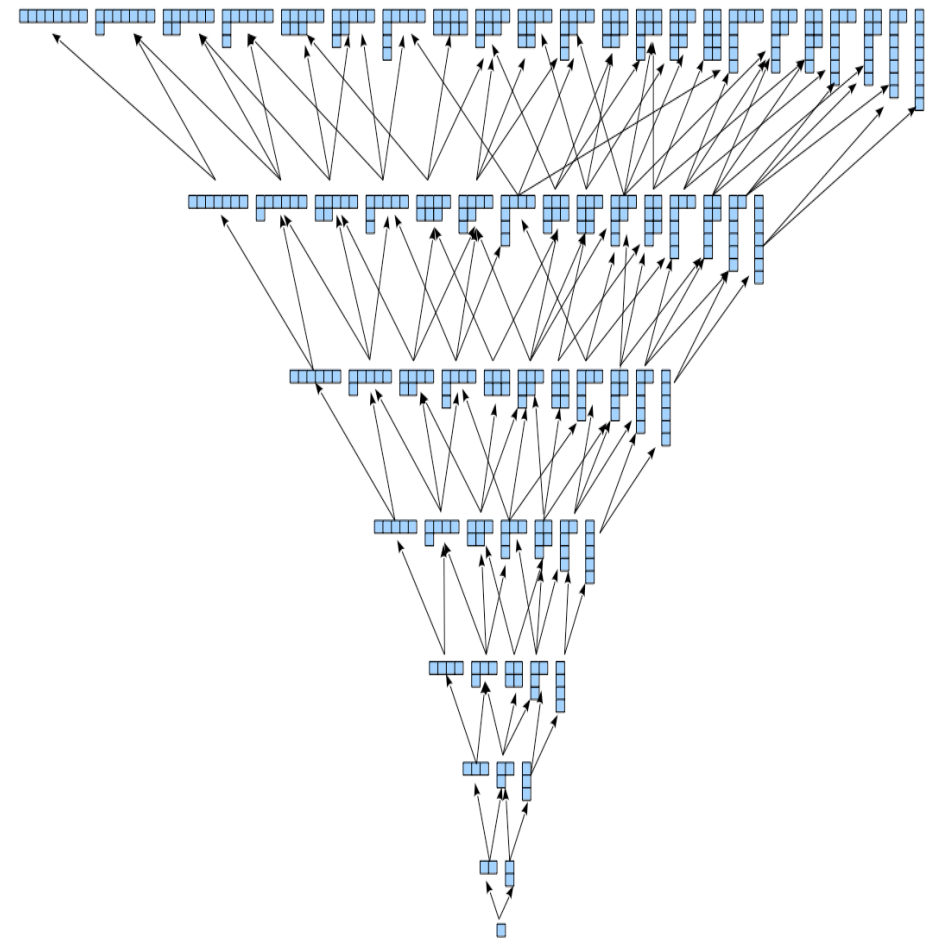
\includegraphics[scale=0.45]{Pictures/youngslattice.png}
                \caption{Young's lattice.}
            \end{figure}

            Young's lattice possess the folling symmetry: the partition $n+n-1+\dots2+1$ of the $n$th triangular number has a Young diagram that looks like a staircase. If we now only keep the elements whose hull is contained in this staircase, we get a subset of Young's lattice. When rank-embedded, this subset clearly has the expected bilateral symmetry of Young's lattice but also a rotational symmetry, which appear more clearly if we move away from this rank-embedding. The rotation group of order $n+1$ acts on this poset\footnote{Partially ordered set.}. Since it has both a bilateral and a rotational symmetry it must also have a dihedral symmetry and, indeed, the dihedral group $\D_{n+1}$ acts faithfully on this set.

            \begin{figure}[H]
                \centering
                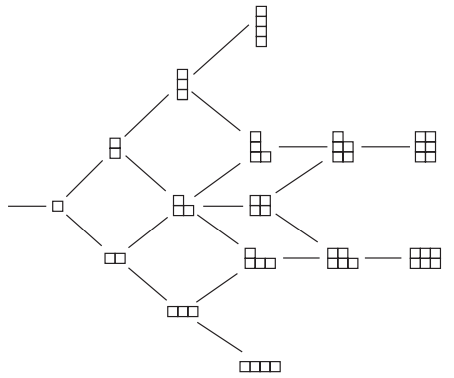
\includegraphics[scale=0.45]{Pictures/suter1.png}
                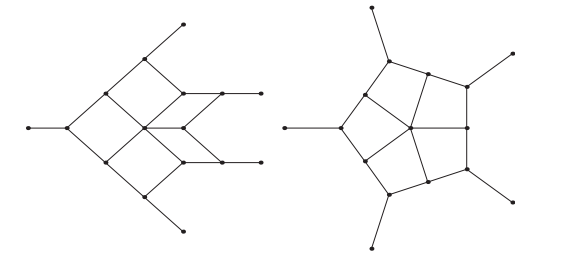
\includegraphics[scale=0.45]{Pictures/suter2.png}
                \caption{Example of dihedral symmetry for $n=4$.}
            \end{figure}

\section{Some derivations}

    \subsection{}\label{app:compsum}

        We want to compute the sum
        \begin{equation}
            \sum^{\lfloor n/3\rfloor}_{a=1}~\left\lfloor \frac{n-3a}{2}+1\right\rfloor = \left\lfloor \frac{n}{3}\right\rfloor + \sum^{\lfloor n/3\rfloor}_{a=1}~\left\lfloor \frac{n-3a}{2}\right\rfloor.
        \end{equation}
        Let us write $n\in\N$ as $n=3m+r$ with $r=0,1$ or $2$ and $m\in\N$. Regardless of $r$, we have $\lfloor n/3\rfloor=m$ and
        \begin{equation}
            \sum^{\lfloor n/3\rfloor}_{a=1}~\left\lfloor \frac{n-3a}{2}\right\rfloor = \sum^{m}_{a=1}~\left\lfloor \frac{3}{2}(m-a)+\frac{r}{2}\right\rfloor = \sum^{m-1}_{a=0}~\left\lfloor \frac{3}{2}a+\frac{r}{2}\right\rfloor.\label{eq:sumfloor}
        \end{equation}
        \begin{itemize}
            \item if $r=0$, then \eqref{eq:sumfloor} becomes
            \begin{equation}
                \sum^{m-1}_{a=0}~\left\lfloor \frac{3}{2}a\right\rfloor = \sum^{m-1}_{a=0}~a+\sum^{m-1}_{a=0}~\left\lfloor \frac{a}{2}\right\rfloor = \frac{(m-1)m}{2}+\sum^{m-1}_{a=0}~\left\lfloor \frac{a}{2}\right\rfloor.
            \end{equation}
            Now if $m$ is even, we have
            \begin{equation}
                \sum^{m-1}_{a=0}~\left\lfloor \frac{a}{2}\right\rfloor = 2\sum^{\left\lfloor \frac{m-1}{2}\right\rfloor}_{a=0}~a = 2\sum^{\frac{m}{2}-1}_{a=0}~a = \left(\frac{m}{2}-1\right)\frac{m}{2}
            \end{equation}
            and if $m$ is odd,
            \begin{equation}
                \sum^{m-1}_{a=0}~\left\lfloor \frac{a}{2}\right\rfloor = 2\sum^{\left\lfloor \frac{m-2}{2}\right\rfloor}_{a=0}~a+\left\lfloor \frac{m-1}{2}\right\rfloor = 2\sum^{ \frac{m-3}{2}}_{a=0}~a+\frac{m-1}{2} = \frac{(m-1)^2}{4}
            \end{equation}
            so
            \begin{equation}
                \sum^{m-1}_{a=0}~\left\lfloor \frac{a}{2}\right\rfloor = 
                \begin{cases}
                    \left(\frac{m}{2}-1\right)\frac{m}{2},\qquad\text{if $m$ is even}\\
                    \frac{(m-1)^2}{4},\qquad\text{if $m$ is odd}
                \end{cases}.\label{eq:suma2floor}
            \end{equation}
            and
            \begin{equation}
                \sum^{m-1}_{a=0}~\left\lfloor \frac{3a}{2}\right\rfloor = 
                \begin{cases}
                    \frac{m(3m-4)}{4},\qquad\text{if $m$ is even}\\
                    \frac{(m-1)(3m-1)}{4},\qquad\text{if $m$ is odd}
                \end{cases}.\label{eq:sum3a2floor}
            \end{equation}
            \item if $r=1$, then \eqref{eq:sumfloor} becomes
            \begin{equation}
                \sum^{m-1}_{a=0}~\left\lfloor \frac{3}{2}a+\frac{1}{2}\right\rfloor = \sum^{m-1}_{a=0}~a+\sum^{m-1}_{a=0}~\left\lfloor \frac{a+1}{2}\right\rfloor = \frac{(m-1)m}{2}+\sum^{m-1}_{a=0}~\left\lfloor \frac{a+1}{2}\right\rfloor
            \end{equation}
            and
            \begin{equation}
                \sum^{m-1}_{a=0}~\left\lfloor \frac{a+1}{2}\right\rfloor = \sum^{m}_{a=1}~\left\lfloor \frac{a}{2}\right\rfloor = \sum^{m}_{a=0}~\left\lfloor \frac{a}{2}\right\rfloor =  
                \begin{cases}
                    \frac{m^2}{4},\qquad\text{if $m$ is even}\\
                    \frac{m^2-1}{4},\qquad\text{if $m$ is odd}
                \end{cases}
            \end{equation}
            by \eqref{eq:suma2floor} so
            \begin{equation}
                \sum^{m-1}_{a=0}~\left\lfloor \frac{3}{2}a+\frac{1}{2}\right\rfloor=
                \begin{cases}
                    \frac{m(3m-2)}{4},\qquad\text{if $m$ is even}\\
                    \frac{3m^2-2m-1}{4},\qquad\text{if $m$ is odd}
                \end{cases}
            \end{equation}
            \item if $r=2$, then \eqref{eq:sumfloor} becomes
            \begin{equation}
                \sum^{m-1}_{a=0}~\left\lfloor \frac{3}{2}a+1\right\rfloor = m+\sum^{m-1}_{a=0}~\left\lfloor \frac{3}{2}a\right\rfloor.
            \end{equation}
            so
            \begin{equation}
                \sum^{m-1}_{a=0}~\left\lfloor \frac{3}{2}a+1\right\rfloor=
                \begin{cases}
                    \frac{3m^2}{4},\qquad\text{if $m$ is even}\\
                    \frac{3m^2+1}{4},\qquad\text{if $m$ is odd}
                \end{cases}
            \end{equation}
            from \eqref{eq:sum3a2floor}.
        \end{itemize}
        Finally, we can write $m=2k$ if $m$ if even and $m=2k+1$ if $m$ is odd in order to distinguish the six different cases. We get
        \begin{align}
            a(n)\equiv\sum^{\lfloor n/3\rfloor}_{a=1}~\left\lfloor \frac{n-3a}{2}+1\right\rfloor&=
            \begin{cases}
                2k+\frac{2k(6k-4)}{4},\qquad\text{if $n=6k$}\\
                2k+\frac{2k(6k-2)}{4},\qquad\text{if $n=6k+1$},\\
                2k+\frac{12k^2}{4},\qquad\text{if $n=6k+2$},\\
                (2k+1)+\frac{2k(6k+2)}{4},\qquad\text{if $n=6k+3$},\\
                (2k+1)+\frac{3(2k+1)^2-2(2k+1)-1}{4},\qquad\text{if $n=6k+4$},\\
                (2k+1)+\frac{3(2k+1)^2+1}{4},\qquad\text{if $n=6k+5$}
            \end{cases}\\
            &=
            \begin{cases}
                3k^2,\qquad\text{if $n=6k$}\\
                3k^2+k,\qquad\text{if $n=6k+1$},\\
                3k^2+2k,\qquad\text{if $n=6k+2$},\\
                3k^2+3k+1,\qquad\text{if $n=6k+3$},\\
                3k^2+4k+1,\qquad\text{if $n=6k+4$},\\
                3k^2+5k+2,\qquad\text{if $n=6k+5$}
            \end{cases}.
        \end{align}
        Starting from $n=1$, the first value of this sequence is : $0,0,1,1,2,3,4,5,7,8,10,12,\dots$. Uppon  further analysis, this correspond to the sequence \href{https://oeis.org/A001399}{\textcolor{blue}{\underline{A001399}}}, that have several interpretations:
        \begin{itemize}
            \item the number of partitions of $n$ into at most 3 parts. This makes sense with our initial problem: finding all the $a,b,c$'s such that $a+b+c=n$,
            \item the number of connected graphs with $3$ nodes and $n$ edges (where multiple edges between the same nodes are allowed),
            \item the number of non-negative solutions to $b+2c+3d=n$,
        \end{itemize}
        as well as many others. Finally, we note that we can simply write
        \begin{equation}
            a(n)=\text{round}\left(\frac{n^2}{12}\right).
        \end{equation}